% EGE 2027, task 13. Source IDs and URLs are kept in comments.
% Editable task bank. Append new BankTask blocks at the end of the document.
\documentclass[12pt,a4paper]{article}
\usepackage{physics-textbook}
\usepackage{graphicx,needspace}
\newif\ifShowSolutions
\ifdefined\TutorEdition
  \ShowSolutionstrue
\else
  \ShowSolutionsfalse
\fi
\newcounter{banktask}
\newcommand{\BankTask}[3]{%
  \refstepcounter{banktask}%
  \Needspace{35mm}\par\medskip\noindent\begin{minipage}{\linewidth}%
  \noindent\textbf{\thebanktask.}\quad #2\par
  \ifShowSolutions
    #3\par
    \ifdefined\TutorEdition
      \ifcsname TutorSource#1\endcsname
        \smallskip{\small\csname TutorSource#1\endcsname\par}%
      \fi
    \fi
  \fi
  \end{minipage}\par\medskip
}
\begin{document}
Справочные величины (если в условии не оговорено иное): $\pi=3{,}14$.



% Source 468FFB: https://ege.fipi.ru/bank/questions.php?search=1&proj=BA1F39653304A5B041B656915DC36B38&qid=468FFB
\BankTask{468FFB}{
\begin{center}
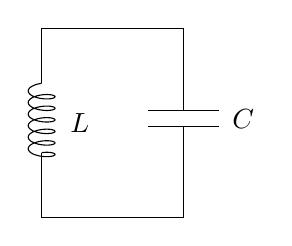
\begin{tikzpicture}[>=stealth,scale=1]
\draw (0,1.7) -- (0,2.4) -- (1.8,2.4) -- (1.8,1.35);
\draw (0,0.7) -- (0,0) -- (1.8,0) -- (1.8,1.15);
\draw (1.35,1.35) -- (2.25,1.35);
\draw (1.35,1.15) -- (2.25,1.15);
\draw (0,0.7) -- (0,0.82);
\draw plot[domain=0:2160,samples=241] ({0.17*sin(\x)},{0.76+0.88*\x/2160+0.06*cos(\x)});
\node[right] at (0.24,1.2) {$L$};
\node[right] at (2.3,1.25) {$C$};
\end{tikzpicture}
\end{center}
В колебательном контуре (см. рисунок) напряжение между обкладками конденсатора меняется по закону $U_C=U_0\cos\omega t$, где $U_0=5\ \text{В}$, $\omega=\pi\cdot10^6\ \text{с}^{-1}$. Определите частоту колебаний силы тока в контуре.

(в $\text{кГц}$).
}{
\smallskip\noindent\textbf{Решение от GPT}\par
Сила тока $I=C\dfrac{dU_C}{dt}=-C U_0\omega\sin\omega t$ имеет ту же циклическую частоту, что и напряжение. Поэтому
\[
\nu=\frac{\omega}{2\pi}=\frac{\pi\cdot10^6}{2\pi}=5\cdot10^5\ \text{Гц}=500\ \text{кГц}.
\]
Ответ: $500$.
}

% Source CFDDFB: https://ege.fipi.ru/bank/questions.php?search=1&proj=BA1F39653304A5B041B656915DC36B38&qid=CFDDFB
\BankTask{CFDDFB}{
Конденсатор, заряженный до разности потенциалов $U$, в первый раз подключили к катушке с индуктивностью $L$, а во второй — к катушке с индуктивностью $4L$. Каково отношение периодов колебаний энергии конденсатора $\dfrac{T_2}{T_1}$ в этих двух случаях? Потерями энергии в контуре пренебречь.
}{
\smallskip\noindent\textbf{Решение от GPT}\par
Энергия конденсатора $W_C=\dfrac{CU^2}{2}\cos^2\omega t$ меняется с периодом $T_W=\dfrac{\pi}{\omega}=\pi\sqrt{LC}$. Следовательно,
\[
\frac{T_2}{T_1}=\sqrt{\frac{4L}{L}}=2.
\]
Ответ: $2$.
}

% Source 91A3F0: https://ege.fipi.ru/bank/questions.php?search=1&proj=BA1F39653304A5B041B656915DC36B38&qid=91A3F0
\BankTask{91A3F0}{
Конденсатор, заряженный до разности потенциалов $U$, в первый раз подключили к катушке с индуктивностью $L_1=L$, а во второй — к катушке с индуктивностью $L_2=4L$. В обоих случаях в получившемся контуре возникли незатухающие электромагнитные колебания. Каково отношение значений полной энергии колебаний $\dfrac{W_2}{W_1}$?
}{
\smallskip\noindent\textbf{Решение от GPT}\par
Полная энергия контура сохраняется и равна начальной энергии заряженного конденсатора: $W=\dfrac{CU^2}{2}$. В обоих случаях ёмкость и начальное напряжение одинаковы, поэтому
\[
\frac{W_2}{W_1}=1.
\]
Ответ: $1$.
}

% Source 0A8805: https://ege.fipi.ru/bank/questions.php?search=1&proj=BA1F39653304A5B041B656915DC36B38&qid=0A8805
\BankTask{0A8805}{
Во сколько раз увеличится частота свободных электромагнитных колебаний в контуре, если площадь пластин конденсатора, входящего в состав контура, уменьшить в \(9\) раз, а индуктивность катушки увеличить в \(4\) раза?
}{
\smallskip\noindent\textbf{Решение от GPT}\par
Ёмкость конденсатора \(C=\varepsilon_0\varepsilon S/d\), поэтому \(C_2=C_1/9\). По формуле Томсона \(\nu=1/(2\pi\sqrt{LC})\), откуда
\[
\frac{\nu_2}{\nu_1}=\sqrt{\frac{L_1C_1}{(4L_1)(C_1/9)}}=\frac{3}{2}=1{,}5.
\]
Ответ: увеличится в \(1{,}5\) раза.
}

% Source 93A417: https://ege.fipi.ru/bank/questions.php?search=1&proj=BA1F39653304A5B041B656915DC36B38&qid=93A417
\BankTask{93A417}{
Конденсатор, заряженный до напряжения \(U_0\), в первый раз подключили к катушке с индуктивностью \(L\), а во второй --- к катушке с индуктивностью \(4L\). В обоих случаях в контуре возникли свободные незатухающие электромагнитные колебания. Каково отношение амплитуд силы тока \(\dfrac{I_{2\max}}{I_{1\max}}\) при этих колебаниях?
}{
\smallskip\noindent\textbf{Решение от GPT}\par
По закону сохранения энергии
\[
\frac{CU_0^2}{2}=\frac{LI_{\max}^2}{2},\qquad I_{\max}=U_0\sqrt{\frac{C}{L}}.
\]
Следовательно, \(\dfrac{I_{2\max}}{I_{1\max}}=\sqrt{\dfrac{L}{4L}}=\dfrac12\).
Ответ: \(0{,}5\).
}

% Source CBF6C6: https://ege.fipi.ru/bank/questions.php?search=1&proj=BA1F39653304A5B041B656915DC36B38&qid=CBF6C6
\BankTask{CBF6C6}{
В двух идеальных колебательных контурах с одинаковой индуктивностью происходят свободные электромагнитные колебания, причём период колебаний в первом контуре \(9\cdot10^{-8}\,\text{с}\), во втором \(3\cdot10^{-8}\,\text{с}\). Во сколько раз амплитудное значение силы тока во втором контуре больше, чем в первом, если максимальный заряд конденсаторов в обоих случаях одинаков?
}{
\smallskip\noindent\textbf{Решение от GPT}\par
Амплитуда силы тока \(I_{\max}=\omega q_{\max}=2\pi q_{\max}/T\). При одинаковых максимальных зарядах
\[
\frac{I_{2\max}}{I_{1\max}}=\frac{T_1}{T_2}=\frac{9\cdot10^{-8}}{3\cdot10^{-8}}=3.
\]
Ответ: в \(3\) раза.
}

% Source 17CD9F: https://ege.fipi.ru/bank/questions.php?search=1&proj=BA1F39653304A5B041B656915DC36B38&qid=17CD9F
\BankTask{17CD9F}{
В таблице показано, как изменялся заряд одной из обкладок конденсатора в идеальном колебательном контуре с течением времени при свободных колебаниях.
\begin{center}
\begin{tabular}{|c|r|r|r|r|r|r|r|r|r|r|}
\hline
$t,\ 10^{-6}\text{ с}$ & $0$ & $1$ & $2$ & $3$ & $4$ & $5$ & $6$ & $7$ & $8$ & $9$ \\
\hline
$q,\ 10^{-6}\text{ Кл}$ & $2{,}0$ & $1{,}42$ & $0$ & $-1{,}42$ & $-2{,}0$ & $-1{,}42$ & $0$ & $1{,}42$ & $2{,}0$ & $1{,}42$ \\
\hline
\end{tabular}
\end{center}
Вычислите индуктивность катушки контура, если ёмкость конденсатора равна $50\text{ пФ}$. Результат в $\text{мГн}$ округлите до целого.
}{
\smallskip\noindent\textbf{Решение от GPT}\par
Заряд повторяет максимальное значение через $T=8\cdot10^{-6}\text{ с}$. По формуле Томсона $T=2\pi\sqrt{LC}$:
\[
L=\frac{T^2}{4\pi^2C}=\frac{(8\cdot10^{-6})^2}{4\cdot3{,}14^2\cdot50\cdot10^{-12}}\approx0{,}03245\text{ Гн}=32{,}45\text{ мГн}.
\]
Ответ: $32\text{ мГн}$.
}

% Source 5F286F: https://ege.fipi.ru/bank/questions.php?search=1&proj=BA1F39653304A5B041B656915DC36B38&qid=5F286F
\BankTask{5F286F}{
В таблице показано, как менялся ток в катушке идеального колебательного контура при свободных электромагнитных колебаниях в этом контуре.
\begin{center}
\begin{tabular}{|c|r|r|r|r|r|r|r|r|r|r|}
\hline
$t,\ 10^{-6}\text{ с}$ & $0$ & $1$ & $2$ & $3$ & $4$ & $5$ & $6$ & $7$ & $8$ & $9$ \\
\hline
$I,\ 10^{-3}\text{ А}$ & $4{,}0$ & $2{,}83$ & $0$ & $-2{,}83$ & $-4{,}0$ & $-2{,}83$ & $0$ & $2{,}83$ & $4{,}0$ & $2{,}83$ \\
\hline
\end{tabular}
\end{center}
Вычислите по этим данным энергию катушки в момент времени $5\cdot10^{-6}\text{ с}$, если ёмкость конденсатора равна $405\text{ пФ}$. Результат в $\text{нДж}$ округлите до целого.
}{
\smallskip\noindent\textbf{Решение от GPT}\par
Из таблицы период $T=8\cdot10^{-6}\text{ с}$, а при $t=5\cdot10^{-6}\text{ с}$ ток $I=-2{,}83\cdot10^{-3}\text{ А}$. Тогда
\[
L=\frac{T^2}{4\pi^2C}=\frac{(8\cdot10^{-6})^2}{4\cdot3{,}14^2\cdot405\cdot10^{-12}}\approx4{,}01\cdot10^{-3}\text{ Гн},
\]
\[
W_L=\frac{LI^2}{2}\approx\frac{4{,}01\cdot10^{-3}\cdot(2{,}83\cdot10^{-3})^2}{2}\approx16\cdot10^{-9}\text{ Дж}.
\]
Ответ: $16\text{ нДж}$.
}

% Source 7CCC09: https://ege.fipi.ru/bank/questions.php?search=1&proj=BA1F39653304A5B041B656915DC36B38&qid=7CCC09
\BankTask{7CCC09}{
На рисунке приведён график зависимости силы тока от времени в колебательном контуре. Сколько раз в течение первых $6\text{ мкс}$ энергия конденсатора достигает минимального значения?
\begin{center}
\begin{tikzpicture}[x=0.85cm,y=0.42cm,>=stealth]
\draw[->] (-1,0)--(7.2,0) node[below] {$t,\text{ мкс}$};
\draw[->] (0,-7)--(0,7) node[left] {$I,\text{ мА}$};
\node[below left] at (0,0) {$0$};
\draw (-0.15,5)--(0.15,5) node[left=5pt] {$5$};
\draw (-0.15,-5)--(0.15,-5) node[left=5pt] {$-5$};
\foreach \x in {1,2,3,4,5,6} \draw (\x,0.15)--(\x,-0.15);
\foreach \x in {1,3,5,6} \node[below] at (\x,-0.3) {$\x$};
\draw[thick,smooth,samples=121,domain=0:6] plot (\x,{5*sin(90*\x)});
\end{tikzpicture}
\end{center}
}{
\smallskip\noindent\textbf{Решение от GPT}\par
Энергия конденсатора $W_C=W-\frac{LI^2}{2}$ минимальна при максимальном модуле тока. На графике это моменты $t=1\text{ мкс}$, $3\text{ мкс}$ и $5\text{ мкс}$. Ответ: $3$ раза.
}

% Source 2C5B74: https://ege.fipi.ru/bank/questions.php?search=1&proj=BA1F39653304A5B041B656915DC36B38&qid=2C5B74
\BankTask{2C5B74}{
На рисунке приведён график зависимости силы тока в идеальном колебательном контуре от времени в процессе свободных электромагнитных колебаний. Каким станет период свободных электромагнитных колебаний в контуре, если конденсатор в этом контуре заменить на другой, ёмкость которого в \(4\) раза меньше?
\begin{center}
\begin{tikzpicture}[x=0.85cm,y=0.42cm,>=stealth]
\draw[->] (-1,0)--(7.25,0) node[below] {\(t,\ \text{мкс}\)};
\draw[->] (0,-6.3)--(0,7) node[left] {\(I,\ \text{мА}\)};
\draw (-0.16,5)--(0.16,5) node[left=5pt] {\(5\)};
\draw (-0.16,-5)--(0.16,-5) node[left=5pt] {\(-5\)};
\node[below left] at (0,0) {\(0\)};
\foreach \t in {1,2,3,4,5,6}\draw (\t,0.15)--(\t,-0.15);
\foreach \t in {1,3,5,6}\node[below] at (\t,-0.35) {\(\t\)};
\draw[thick,domain=0:6,samples=121] plot (\x,{5*sin(90*\x)});
\end{tikzpicture}
\end{center}
(в $\text{мкс}$).
}{
\smallskip\noindent\textbf{Решение от GPT}\par
По графику соседние максимумы тока соответствуют \(t_1=1\,\text{мкс}\) и \(t_2=5\,\text{мкс}\), поэтому \(T=t_2-t_1=4\,\text{мкс}\). По формуле Томсона \(T=2\pi\sqrt{LC}\). При \(C'=C/4\) получаем \(T'=T\sqrt{C'/C}=T/2=2\,\text{мкс}\).
Ответ: \(2\,\text{мкс}\).
}

% Source 1732F3: https://ege.fipi.ru/bank/questions.php?search=1&proj=BA1F39653304A5B041B656915DC36B38&qid=1732F3
\BankTask{1732F3}{
Луч света падает на плоское зеркало. Угол отражения равен \(30^\circ\). Определите угол между падающим и отражённым лучами.
}{
\smallskip\noindent\textbf{Решение от GPT}\par
По закону отражения угол падения равен углу отражения: \(\alpha=\beta=30^\circ\). Угол между лучами \(\varphi=\alpha+\beta=60^\circ\).
Ответ: \(60^\circ\).
}

% Source 4D7B06: https://ege.fipi.ru/bank/questions.php?search=1&proj=BA1F39653304A5B041B656915DC36B38&qid=4D7B06
\BankTask{4D7B06}{
Луч света падает на плоское зеркало. Угол между падающим и отражённым лучами равен \(30^\circ\). Чему равен угол между падающим лучом и зеркалом?
}{
\smallskip\noindent\textbf{Решение от GPT}\par
Углы падения и отражения равны, поэтому угол падения \(\alpha=30^\circ/2=15^\circ\). Угол между падающим лучом и зеркалом равен \(90^\circ-\alpha=75^\circ\).
Ответ: \(75^\circ\).
}

% Source 758809: https://ege.fipi.ru/bank/questions.php?search=1&proj=BA1F39653304A5B041B656915DC36B38&qid=758809
\BankTask{758809}{
На шахматной доске на расстоянии двух клеток от вертикального плоского зеркала стоит слон. На сколько клеток увеличится расстояние между слоном и его изображением, если фигуру на три клетки отодвинуть от зеркала?
}{
\smallskip\noindent\textbf{Решение от GPT}\par
Изображение находится на таком же расстоянии за зеркалом, как предмет перед ним, поэтому расстояние между ними равно \(D=2d\). Увеличение расстояния составит \(\Delta D=2\Delta d=2\cdot3=6\) клеток. Ответ: \(6\) клеток.
}

% Source F3157e: https://ege.fipi.ru/bank/questions.php?search=1&proj=BA1F39653304A5B041B656915DC36B38&qid=F3157e
\BankTask{F3157e}{
Точечный источник света находится на расстоянии \(75\ \text{см}\) от плоского зеркала. На сколько уменьшится расстояние между источником и его изображением, если, не поворачивая зеркала, придвинуть его к источнику на \(25\ \text{см}\) (в $\text{см}$)?
}{
\smallskip\noindent\textbf{Решение от GPT}\par
Расстояние между источником и изображением равно \(D=2d\). Первоначально \(D_1=2\cdot75=150\ \text{см}\), после перемещения зеркала \(D_2=2(75-25)=100\ \text{см}\). Уменьшение: \(D_1-D_2=50\ \text{см}\). Ответ: \(50\ \text{см}\).
}

% Source 0439A7: https://ege.fipi.ru/bank/questions.php?search=1&proj=BA1F39653304A5B041B656915DC36B38&qid=0439A7
\BankTask{0439A7}{
Точечный источник света расположен перед плоским зеркалом на расстоянии \(1{,}2\ \text{м}\) от него. На сколько необходимо приблизить зеркало, не поворачивая его, к источнику, чтобы расстояние между источником и его изображением в зеркале уменьшилось в \(2\) раза (в $\text{м}$)?
}{
\smallskip\noindent\textbf{Решение от GPT}\par
Расстояние между источником и изображением равно \(D=2d\). Чтобы оно уменьшилось в \(2\) раза, расстояние до зеркала должно стать \(d_2=d_1/2=0{,}6\ \text{м}\). Перемещение зеркала: \(x=d_1-d_2=1{,}2-0{,}6=0{,}6\ \text{м}\). Ответ: \(0{,}6\ \text{м}\).
}

% Source 507D42: https://ege.fipi.ru/bank/questions.php?search=1&proj=BA1F39653304A5B041B656915DC36B38&qid=507D42
\BankTask{507D42}{
Предмет расположен на главной оптической оси тонкой собирающей линзы. Оптическая сила линзы \(D=5\,\text{дптр}\). Изображение предмета действительное, увеличение (отношение высоты изображения предмета к высоте самого предмета) \(k=2\). Найдите расстояние между предметом и его изображением. Ответ выразите в сантиметрах. (в $\text{см}$).
}{
\smallskip\noindent\textbf{Решение от GPT}\par
Фокусное расстояние \(F=1/D=0{,}2\,\text{м}=20\,\text{см}\). Обозначим расстояния от линзы до предмета и изображения через \(a\) и \(b\). Тогда \(b/a=k=2\), а по формуле тонкой линзы
\[\frac1F=\frac1a+\frac1b=\frac{3}{2a}.\]
Отсюда \(a=30\,\text{см}\), \(b=60\,\text{см}\). Предмет и действительное изображение находятся по разные стороны линзы, поэтому \(l=a+b=90\,\text{см}\). Ответ: \(90\,\text{см}\).
}

% Source AC9F7A: https://ege.fipi.ru/bank/questions.php?search=1&proj=BA1F39653304A5B041B656915DC36B38&qid=AC9F7A
\BankTask{AC9F7A}{
Фокусное расстояние собирающей линзы равно \(40\,\text{см}\). На каком расстоянии от линзы находится предмет, если линза даёт его мнимое изображение на расстоянии \(60\,\text{см}\) от линзы (в $\text{см}$)?
}{
\smallskip\noindent\textbf{Решение от GPT}\par
Для собирающей линзы \(F=40\,\text{см}\), для мнимого изображения \(b=-60\,\text{см}\). По формуле тонкой линзы
\[\frac1a=\frac1F-\frac1b=\frac1{40}+\frac1{60}=\frac1{24}\,\text{см}^{-1}.\]
Ответ: \(a=24\,\text{см}\).
}

% Source B81EB6: https://ege.fipi.ru/bank/questions.php?search=1&proj=BA1F39653304A5B041B656915DC36B38&qid=B81EB6
\BankTask{B81EB6}{
В тонкой рассеивающей линзе получено уменьшенное в \(3\) раза изображение предмета. Определите модуль фокусного расстояния линзы, если изображение предмета находится на расстоянии \(f=16\,\text{см}\) от линзы. (в $\text{см}$).
}{
\smallskip\noindent\textbf{Решение от GPT}\par
Изображение в рассеивающей линзе мнимое: \(b=-16\,\text{см}\). Увеличение \(k=|b|/a=1/3\), поэтому \(a=48\,\text{см}\). По формуле тонкой линзы
\[\frac1F=\frac1a+\frac1b=\frac1{48}-\frac1{16}=-\frac1{24}\,\text{см}^{-1}.\]
Следовательно, \(F=-24\,\text{см}\). Ответ: \(|F|=24\,\text{см}\).
}

% Source 402B55: https://ege.fipi.ru/bank/questions.php?search=1&proj=BA1F39653304A5B041B656915DC36B38&qid=402B55
\BankTask{402B55}{
Предмет высотой \(6\,\text{см}\) расположен на горизонтальной главной оптической оси тонкой собирающей линзы. Оптическая сила линзы \(5\,\text{дптр}\). Действительное изображение предмета находится на расстоянии \(30\,\text{см}\) от оптического центра линзы. Найдите высоту изображения предмета. (в $\text{см}$).
}{
\smallskip\noindent\textbf{Решение от GPT}\par
Фокусное расстояние линзы \(F=1/D=0{,}2\,\text{м}=20\,\text{см}\). По формуле тонкой линзы расстояние до предмета
\[
a=\frac{Fb}{b-F}=\frac{20\cdot30}{30-20}=60\text{ см}.
\]
Высота изображения \(H=h\,b/a=6\cdot30/60=3\,\text{см}\). Изображение перевёрнутое.
\(\boxed{3\text{ см}}\).
}

% Source 97F253: https://ege.fipi.ru/bank/questions.php?search=1&proj=BA1F39653304A5B041B656915DC36B38&qid=97F253
\BankTask{97F253}{
Оптическая сила тонкой собирающей линзы равна \(1\,\text{дптр}\). Точечный источник света, расположенный на главной оптической оси линзы, удалён от неё на три фокусных расстояния. На каком расстоянии от линзы находится изображение источника (в $\text{м}$)?
}{
\smallskip\noindent\textbf{Решение от GPT}\par
Фокусное расстояние \(F=1/D=1\,\text{м}\), расстояние до источника \(a=3F\). По формуле тонкой линзы
\[
\frac1b=\frac1F-\frac1{3F}=\frac2{3F},\qquad b=\frac{3F}{2}=1{,}5\text{ м}.
\]
\(\boxed{1{,}5\text{ м}}\).
}

\end{document}
